\chapter{Learning useful representations of data}\label{ch:learningrepresentations}



In this chapter, we introduce the basic ideas from representation learning.
We identify properties of \textit{good data representations} and illustrate common representation learning approaches.
Finally, we summarise the main ideas within the relational representation learning literature.



\section{Introduction}


As we have seen in Section \ref{sec:intro_ml} of Chapter \ref{ch:introduction}, machine learning intuitively corresponds to \textit{discovering} a decision function \textit{f} mapping the input data $X$ to some target concept $y$:

\begin{equation}
	f(X) = y.
	\label{eq:ml}
\end{equation}


This also illustrates why we care so much about the representation of data: if the relevant information in $X$ is insufficiently captured or represented, whatever \textit{f} we learn  is doomed to be a bad one.
As one relies on \gls{ml} in scenarios when one has little or no knowledge of \textit{f}, it is very difficult, if not impossible, to know in advance which information is relevant for the mapping.
Deploying \gls{ml} solution in practice, thus, requires a lot of manual work just to identify the relevant information for the task.
Insufficiently captured information does not imply that the relevant information is not present, but instead is not represented explicitly enough.
A typical example is illustrated in Figure \ref{fig:transform} in which blue dots are difficult to separate from red ones in the original data representation, but transforming the data into a new latent representation makes them easy to separate.


\begin{figure}
	\centering
	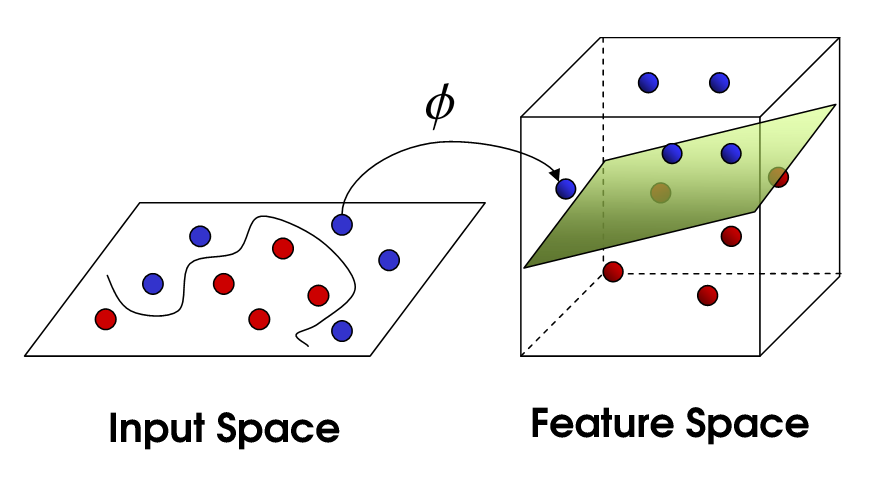
\includegraphics[width=.8\linewidth]{insufficientrepresentation}
	\caption[A choice of problem representation matters]{A choice of problem representation matters - having a good and informative features can simplify learning\label{fig:transform}}
\end{figure}

A pleasing property of introducing a representation learning component in a \gls{ml} pipeline is that is \textit{surpasses the limitation of fixed data representation}.
It thus generalises the machine learning equation (Equation \ref{eq:ml}) to:

\begin{equation}
	f(m(X)) = y
\end{equation}


where, in addition to the decision functions \textit{f}, we include the representation mapping function \textit{m}.
Moreover, several mapping function can be \textit{stacked} together to perform multiple representation learning steps.







\section{Representation learning principles}


The core focus of representation learning is on \textit{learning} the function(s) \textit{m}$_{(i)}$.
By the time of writing of this thesis, several thousands of different representation learning methods exist in the literature \cite{Goodfellow2016}.
In this section, we illustrate the principles of representation learning on a few prototypical approaches.


\subsection{Artificial neural networks}



\newglossaryentry{ann}{name={ANN},description={Artificial Neural Networks}}
Representation learning as a field has risen from the advances in \textit{artificial neural networks} (\gls{ann}).
Until this day, almost all representation learning methods are developed within the framework of \gls{ann}s.

\begin{figure}
	\centering
	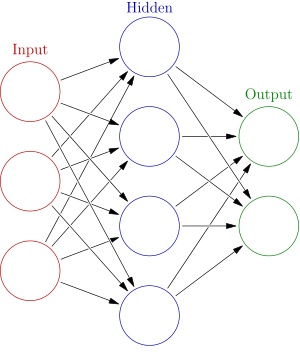
\includegraphics[width=.5\linewidth]{ann}
	\caption[Illustration of an artificial neural networks]{An artificial neural network consists of \textit{input neurons} (in red) that represent the data, \textit{output neuron} (green) representing the target concept and \textit{hidden neurons} performing the feature creating step}
	\label{fig:ann}
\end{figure}


\gls{ann} (Figure \ref{fig:ann}) is a simple mathematical formalisation for machine learning, inspired by the topology of  \textit{human brain}.
It consists of a \textit{network} of mutually connected \textit{artificial neurons}, also known as \textit{perceptrons} (circles in Figure \ref{fig:ann}).
The interactions between neurons are dictated by their connections (edges connecting circles in Figure \ref{fig:ann}).




An \gls{ann} in Figure \ref{fig:ann} consists of three \textit{layers}: an \textit{input layer} which takes the data $X$, an \textit{output layer} capturing the target concept $y$ and a \textit{hidden layer} performing the representation transformation.
\gls{ann} operates by activating neurons in different amounts depending on the input data -- similar to the human brain.
Each neuron in the hidden layer is connected to all of the input neurons but with different \textit{strengths} of connections.
In formal terms, the amount of activation of any individual neuron equals

\begin{equation}
	a(X) = n(\sum_{i=1}^N w_i \times x_i)
\end{equation}

where $w_i$ stands for the strength of the connection, and $x_i$ is the value of an input neuron.
The function \textit{n} is any non-linear function determining the activation based on the weighted sum of the activation of the input neurons, i.e., the data.




The task of learning \gls{ann}s is the one of learning the strengths of connections given a fixed structure of an \gls{ann}s.
Once learned, the activation's of the neurons in the hidden layer represents the new representation of data.


This flavour of representation learning belongs to the \textbf{supervised} branch, i.e.,  new representation tailored specifically for the given task ($y$).




\subsection{Auto-encoders}


A very different approach to learning representations are \textit{auto-encoders} \cite{Hinton504}.
Auto-encoders belong to the \textbf{unsupervised} branch of representation learning methods which do not consider a particular supervised or target information when learning representations.
A benefit of unsupervised representation learning is that the new representations can be used for many tasks as they are not tailored to a certain task.


Learning new representations in an unsupervised way is substantially more difficult than the supervised case.
Given the labelled information, one can verify how useful every feature in the new representation is  by, for instance, evaluation to which extent each feature contributes towards distinguishing different target labels.
In the unsupervised case, we have no access to such information.
The question then is: \textit{What constitutes a good representation if we don't know the target task?}


\begin{figure}
	\centering
	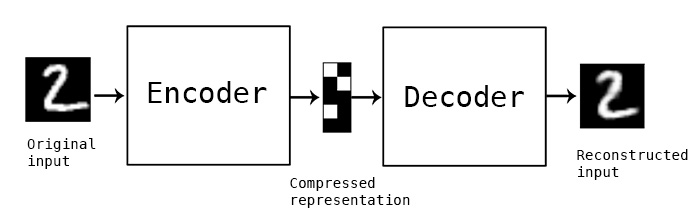
\includegraphics[width=.8\linewidth]{ae}
	\caption[Illustration of the auto-encoding principle]{\textbf{Illustration of the auto-encoding principle.} An auto-encoder \textit{encoding} the provided input image to a \textit{compressed representation} and \textit{decodes} it back to the original feature space}
	\label{fig:ae}
\end{figure}



Auto-encoders introduce a practical way to circumvent tackling this difficult question first.
Auto-encoders are \gls{ann}s that learn data representation by trying to compress the original data such that the original data can be reliably reconstructed from the compressed representation.
Thus, auto-encoders \textit{tricks} the supervised learning method into an unsupervised one.
Two parts of an auto-encoder (Figure \ref{fig:ae}) are an \textit{encoder}, mapping the original data to a new representation, and a \textit{decoder} mapping the latent representation of data back to the original data representation.
It is important to note that training auto-encoders does not require any change in learning \gls{ann}s, except for the requirement that the \gls{ann} reconstructs its own input $y \approx X$.




The key in successfully learning representation with auto-encoders lies in imposing certain constraints on the hidden layer of the auto-encoder.
Otherwise, without the constraints, nothing prevents the auto-encoders to learn the \textit{identity mapping} which would guarantee the perfect reconstruction.
The most common way of preventing the learning of identity mapping is to force the auto-encoders to be \textit{compressive}; this is achieved by restricting the dimension of the hidden layer to be \textit{smaller} than the dimension of the input data.
This way, the auto-encoder is forced to exploit the patterns in data in order to maximise the reconstruction from the latent representation.







\subsection{Properties of good data representation}
\label{ch3:sec:properties}


The success of representation learning opened many novel research questions, one of the most important ones being: \textit{what constitutes a good data representation?}
Bengio and LeCun \cite{Bengio2013RLR} argue that explicitly dealing with representations is important and beneficial because representation can be convenient to express general priors about the real worlds.
The priors we are interested in should not be task-specific, but likely useful for many different \gls{ai} tasks.
Investigating such general priors has largely shaped the representation learning research over the past decade, and could likely be its most important contribution.
Some of the general-purpose representation priors are the following.



\paragraph{\textbf{Smoothness and locality}}
The most basic representation prior is \textit{smoothness}: learning a function $f$ is locally consistent, i.e., if $ x \approx y$ then $f(x) \approx f(y)$.
This property simply states that predictions should be \textit{robust} and generalise to local regions of feature space, reflected in a requirement that similar examples should have a similar prediction.
%This can be also interpreted as \textit{robustness}: small alteration of instance's features should not change the prediction of an \gls{ml} system.




\paragraph{\textbf{Multiple explanatory factors}}
The generative data distribution typically comprises several \textit{underlying factors}, and learning something about one of the factors generalises to many configurations of the other factors.
This prior gave rise to one of the pillars of representation learning -- a  \textit{distributed representation}.
The concept of distributed representation directly relates the quality of representation to its expressivity: good representations are \textit{expressive}, meaning that a reasonably-sized representation can capture a huge number of possible input configurations.
An intuitive way to think about the capacity of the representation is comparing the number of parameters a representation requires to the number of regions it can represent.
On the lower end, \textit{one-hot} representations common among many \gls{ml} methods can represent $N$ regions with $N$ parameters.
On the upper end, distributed representations can represent up to $2^N$ regions with $N$ parameters.
Representation learning advertises learning of representation with the latter properties, as the gain in expressivity is evident.



\paragraph{\textbf{Hierarchical organisation of explanatory factors}}
The knowledge we pose about the world around us is not simply a collection of facts, but a hierarchically organised system.
Many concepts are defined in terms of other concepts, structured in a hierarchy so that \textit{low-level concepts} which can be directly observed in the real world constitute the foundations of the hierarchy while the more abstract concepts appear in the higher levels of the hierarchy.
The advantage of such hierarchically structured knowledge is that they promote \textit{concept re-use} between the levels of hierarchy, which even further increases the expressivity of the representation.
Moreover, concept re-use allows one to express complex concepts \textit{compactly}.
This is even more evident considering the \textit{depth} of the hierarchy which indicates the number of levels of abstraction within the hierarchy, i.e., the number of steps from the concept at the bottom of the hierarchy to the most abstract concept.
As the number of paths between concepts of different levels of abstractions (i.e. ways to re-use different parts) increases exponentially with the depth, theoretical results have shown that a deep representation can be exponentially more efficient than one that is insufficiently deep \cite{Hastad:1986:AOL:12130.12132,89582,Bengio:2011:EPD:2050345.2050349}





\paragraph{\textbf{Shared factors across tasks}}
Given many learning tasks of interest, a good data representation contains factors that are shared among many tasks.
More precisely, each factor in a representation helps to explain many several different tasks.
This does not necessarily work for supervised tasks: given a data $X$ and a target task $Y$, a representation useful for explaining the data generating distribution $P(X)$ tend to be useful when learning a predictive task $Y$ given $X$, $P(Y|X)$.
If this property if fulfilled, it allows having a single data representation for different tasks which can have many practical benefits for big data, e.g., storage.
Moreover, it also allows for sharing statistical strength across tasks.




\paragraph{\textbf{Sparsity}}
Sparsity refers to the notion that for each individual data point only a small subset of factors is relevant.
In practical terms, this means that latent representation of each example contains only a small number of \textit{non-zero features}.
Sparsity enforces latent representation to partition the instance space in local regions for which only a small number of factors are relevant.
This also makes the representation more robust to noise; as only a small number of factors matters, noise is more likely to affect the irrelevant factors.




\paragraph{\textbf{Natural clustering and manifolds}}
Humans have named categories, they name things, and one of the prevalent hypothesis in neuroscience is that this is due to the statistical regularities in the world we perceive.
This means that categories \textit{naturally group} into regions that tend to be well separated and non-overlapping.
The regions where different categories lie are therefore \textit{more dense} than the regions between categories; these regions are known as \textit{data manifold}.
Many of the representation learning approaches try to exploit this property.





\paragraph{\textbf{Simplicity of factor dependencies}}
A good data representation suitable for high-level reasoning should make the final task, e.g. prediction, simple(er) to solve.
In practical terms, that means that the dependencies between the factors at the last level of representation hierarchy should be simple and \textit{linear}.
From an \gls{ml} perspective, a final data representation should allow a user to use a simple method, such as linear or logistic regression, to learn a successful predictor.












\section{Learning representations of relational data}


The few examples discussed in the previous section consider learning representation from tabular data only.
In this section, we provide a brief overview of the main ideas present in transferring these ideas towards relational data.


\subsection{Knowledge graph embeddings}

\newglossaryentry{kge}{name={KGE},description={Knowledge Graph Embeddings}}

By far the largest group of methods for representation learning with relational data are \textit{knowledge graph embeddings} (\gls{kge}).
Knowledge graph embeddings, in their core, approximate the symbolic data (such as the one described in Chapter \ref{ch:learninglogic}) with vectors and/or matrices in the Euclidean space.
For instance, Figure \ref{fig:emb} illustrates a small part of a large knowledge graph capturing the information about Barack and Michelle Obama.
\gls{kge}s replace entities, the constant symbols such as \textit{barack} and \textit{michelle}, with $n$-dimensional vectors and relations, the predicate symbols such as \textit{wasBornIn} and \textit{isMarriedTo}, with either vectors or matrices.

 \begin{figure}
	\centering
	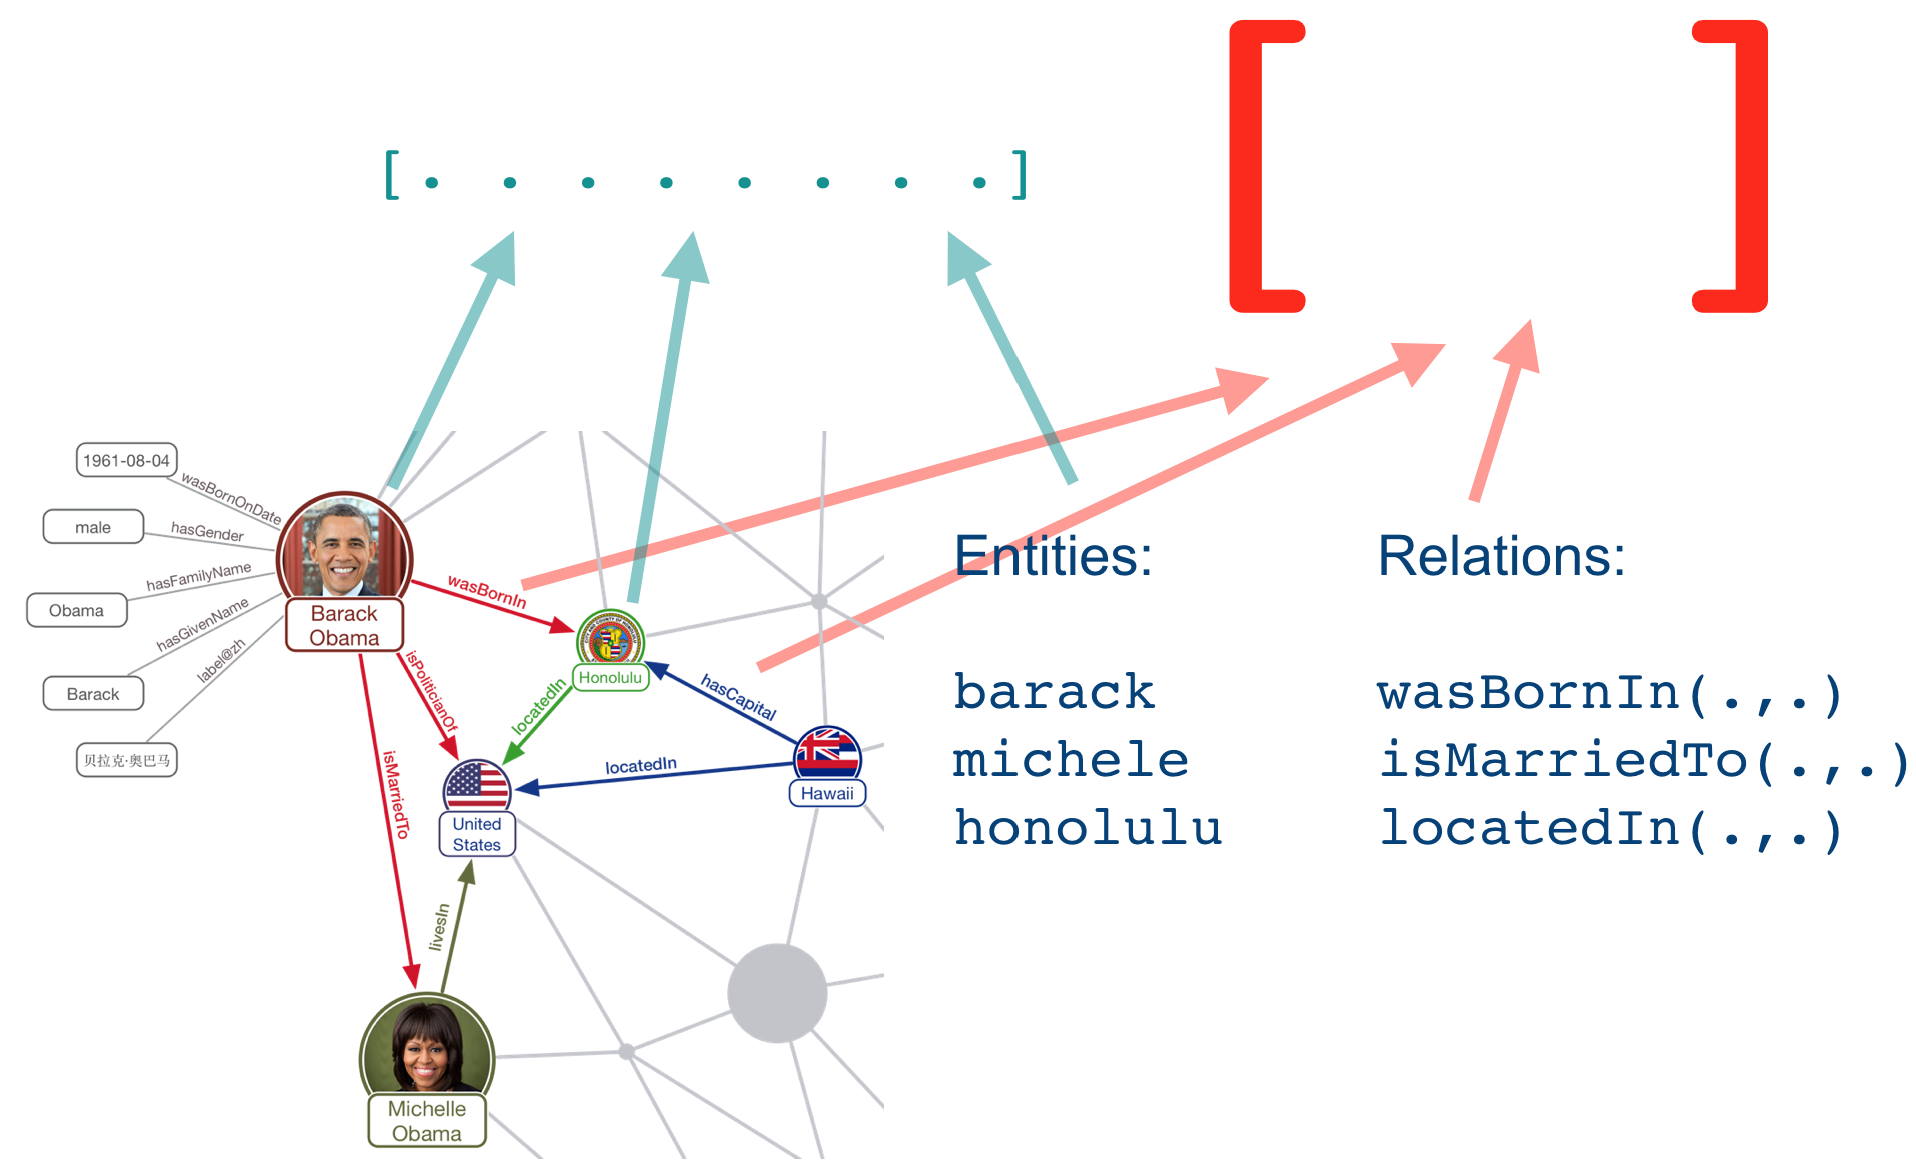
\includegraphics[width=.8\linewidth]{illustrationembeddings}
	\caption[Representing relational data with embeddings]{\textbf{Representing relational data with embeddings} Embedding approaches map entities (such as \textit{barack} and \textit{michelle}) to vectors in the Euclidean space and relations (such as \textit{wasBornIn}) to vectors of matrices}
	\label{fig:emb}
\end{figure}




The representation learning task of \gls{kge}s is the one of learning the numerical representation of symbols (Figure \ref{fig:emb}).
To evaluate the \textit{fitness} of a numerical representation, \gls{kge} associate a \textit{score} with each fact of the form \textit{predicate(subject,object)}.
The vast variety of \gls{kge} methods comes from simply modifying the score function.
The existing score functions largely belong to two groups of approaches:

\begin{itemize}
	\item \textbf{Translational approaches:} these approaches interpret relations as \textit{translations} between objects. That is, the score measure how well the vector representation of the \textit{head} object translates to the vector representation of the \textit{tail} object through the given \textit{relation}: \textit{head} + \textit{relation} $\approx$ \textit{tail}:
		\begin{equation}
			s(h,r,t) = - || \mathbf{e}_{h} + \mathbf{e}_{r} - \mathbf{e}_{t} ||
		\end{equation}
		Examples of such approaches are \textit{transE} \cite{Bordes:2013:TEM} and its variants \cite{Lin:2015:LER:2886521.2886624,nguyen-EtAl:2016:N16-1,Arbelaitz:2013,P15-1067}

	\item \textbf{Latent feature matching:} these approaches measure how well the \textit{latent features} of objects, i.e. the individual components in vector representations, match. This is typically done by a pairwise comparison of feature values:
	 	\begin{equation}
	 		s(h,r,t) = \mathbf{e}_{h} \cdot \mathbf{R} \cdot \mathbf{e}_{t}^{\text{T}}
	 	\end{equation}
	 	A typical representatives of this \gls{kge} branch are \textit{RESCAL} \cite{Nickel2011}, \textit{DistMult} \cite{YangYHGD14a} and \textit{complEX} \cite{trouillon2016complex}.
\end{itemize}


The main advantage of \gls{kge}s is that, in principle complex, logical reasoning is replaced with a simple algebraic computation.
This makes \gls{kge}s a very scalable approach for relational learning.
The main limitation of these methods is that they only approximate the original structured data, and it is difficult to quantify the \textit{quality} of the approximation.
Moreover, as the learning problem is defined in terms of \textit{scores} of the facts, \gls{kge}s cannot easily incorporate  long-range dependencies between objects.
In contrast to \gls{srl} models such as Problog and Markov logic networks which can perform many types of inferences, \gls{kge}s can only be used for ranking the possible answer for a knowledge base completion tasks.




 % TODO: add graph neural networks






\subsection{Capturing data properties with random walks}


\gls{kge}s aim at completely replacing the relational or graph structure information with vectors.
An alternative approach is to use parts of the relational information directly as features.


One such approach is \textit{DeepWalk} \cite{Perozzi:2014:DOL:2623330.2623732}, which combines the ideas of random walks in a graph with the language modelling methodologies.
In order to learn the vector representations of objects in a graph, \textit{DeepWalk} first performs random walks collecting the sequences of nodes.
The obtained node sequences are treated as \textit{sentences} in a document and popular word embedding method of  \textit{SkipGram} \cite{NIPS2013_Skipgram} which learns word embeddings based on the co-occurrences of words.



As \textit{DeepWalk} uses sequences of nodes of a graph, it is inherently \textit{transductive} and the method cannot be directly applied in inductive settings.
To circumvent the issues, methods such as \textit{Path-ranking Algorithm} \cite{lao2010pra,Lao:2011:RWI:2145432.2145494}, \textit{Discriminative Gaifman models} \cite{Niepert:2016:DGM:3157382.3157479} and \textit{Relational Restricted Boltzmann machines} \cite{KaurILP17} rely on random walks like \textit{DeepWalk} but use sequences of the traversed edge labels instead of nodes.
Therefore, these methods can be easily applied in the inductive settings.



\textit{Path-ranking Algorithm} is a model oriented towards the knowledge base completion tasks and it considers the task of ranking target nodes $y$ with respect to a query node $x$.
It starts by enumerating a large collection of length-bounded paths, followed by estimation of the conditional probability distribution for each rule.
The discovered rules are considered to be the \textit{ranking experts}, which are combined by means of logistic regression.




\textit{Discriminative Gaifman models} introduces a novelty of learning \textit{ego-centric} representations of relational data by first extracting small bounded neighbourhoods (so-called the \textit{Gaifman graph}~\cite{GAIFMAN1982105}) around each object in the data followed by extraction of relational features from the bounded neighbourhoods.
The discovered relational features are associated with the elements in a vector and are encoding the existence of the features or the count of the relational features within the bounded neighbourhood.
This offers a trade-off between efficiency (how \textit{fast} we can do the learning) and expressiveness (how much we can \textit{express} with the given language).



\textit{Relational Restricted Boltzmann machines} follow the idea very similar to the Gaifman models.
The main difference is that they do not consider the relational features only within the Gaifman graph but within the entire data.
Moreover, Relational Boltzmann machines use pathfinding as a relational features extraction method, while the Gaifman models can in principle use any \gls{ilp} learning method.






\subsection{Logic-based approaches}


\newglossaryentry{lrnn}{name={LRNN},description={Lifted Relational Neural Network}}
\newglossaryentry{relnn}{name={RelNN},description={Relational Neural Network}}
Previously discussed embeddings approaches are by far the predominant paradigm when learning latent representations of relational data.
Developing logic-based methods for relational representation learning attracted significantly less attention, but offers many benefits as discussed in Chapter~\ref{ch:introduction}.
Two examples are \textit{Lifted relational neural networks} (\gls{lrnn}) \cite{LRNN} and \gls{relnn} \cite{Kazemi2018}.

\begin{figure}
	\medskip
	\centering
	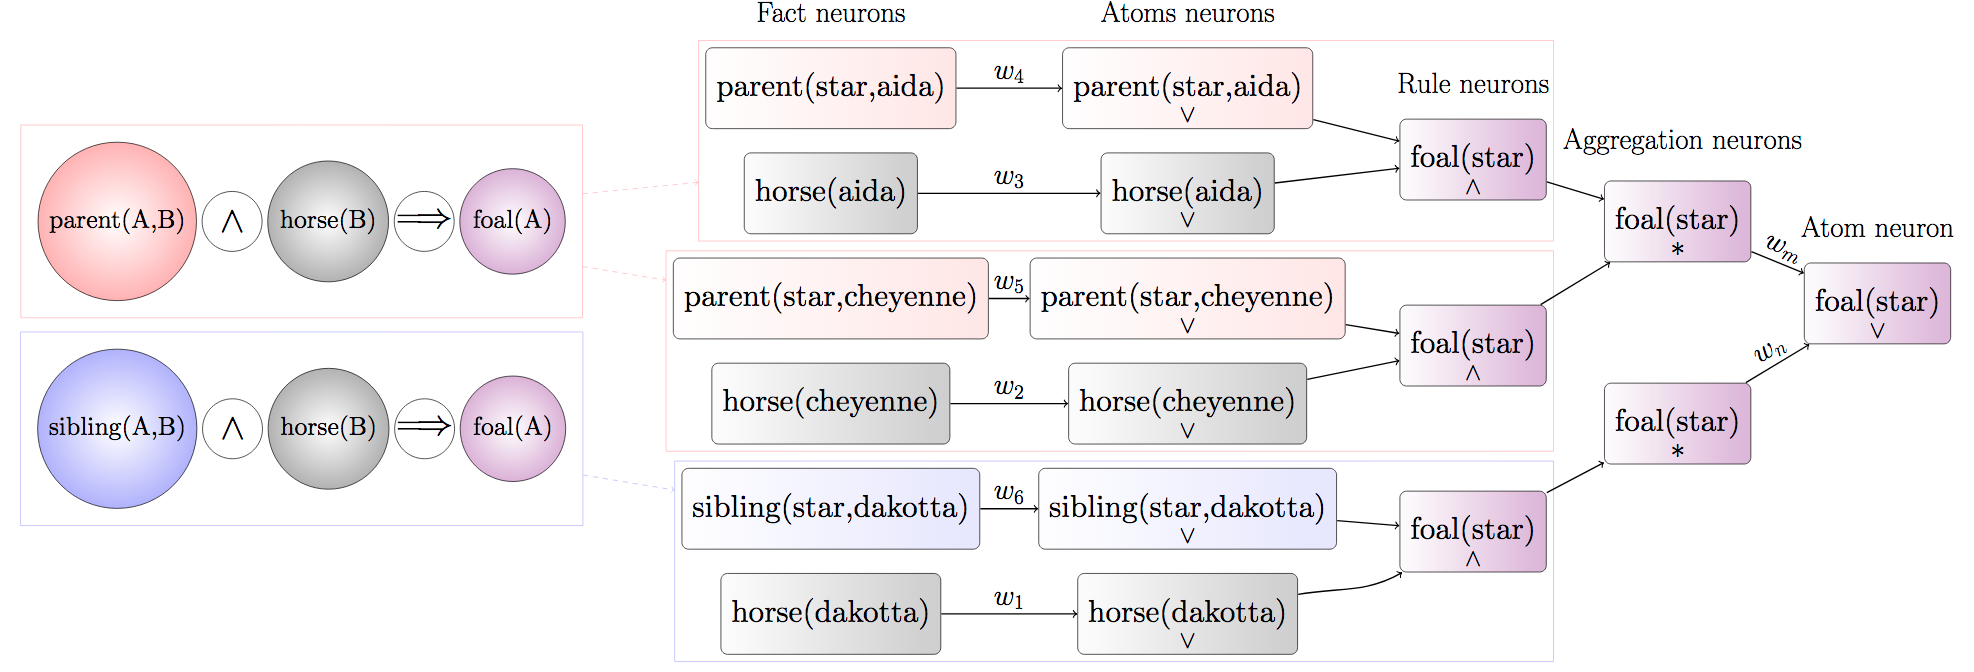
\includegraphics[width=.9\linewidth]{LRNN}
	\caption[Lifted relational neural networks]{Lifted relational neural networks provide a \textit{template} model (left) for constructing a grounded relational neural network (right)\label{fig:lrnn}}
\end{figure}



\gls{lrnn}s provide a template language that maps  fuzzy logical rules and data to big neural networks, in very much the same way how Markov logic networks provide a language to map complex \gls{srl} models to Markov networks.
The structure of the model, i.e.,  the logical rules, therefore define the structure of a neural network (Figure~\ref{fig:lrnn}, left).
The mapping between logical and neural constructs is dictated via different types of neurons:
\begin{itemize}
	\item each ground fact is associated with a \textit{fact neuron} taking no inputs and with value $w_k$ (corresponding to a weight in a \gls{ann}) as output
	\item each ground atom is associated with an \textit{atom neuron}
	\item each ground rule is associated with a \textit{rule neuron}
	\item different instantiations of the same rule are handled through \textit{aggregation neurons}.
\end{itemize}
The final structure of the \gls{lrnn} is dictated by the data (Figure~\ref{fig:lrnn}, right).
Additionally, parameter learning is inherited from the neural networks, as well as the inference.




\gls{relnn} takes a different approach and constructs relational neural networks out of relational logistic regression models as a basic primitive (Figure~\ref{fig:relnn}).
This is very similar to the functioning of \gls{ann}s in which an activation of each hidden neuron can be seen as a prediction made through the logistic regression, but with a difference that the features are relational.
For instance, $S1(u)$, $S2(u)$ and $S3(u)$ predicates in Figure~\ref{fig:relnn} are relational logistic regression models jointly defining the relational neural network.



\begin{figure}
	\centering
	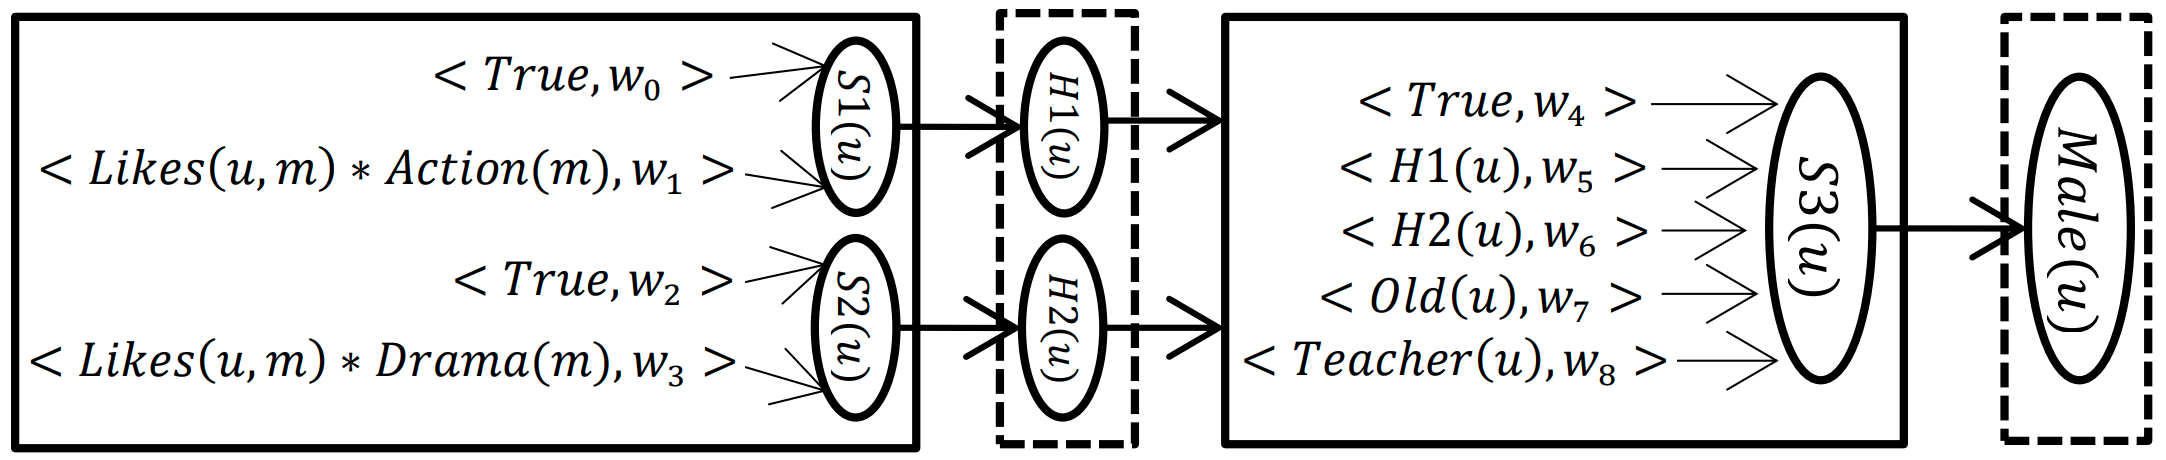
\includegraphics[width=.8\linewidth]{rlr}
	\caption[Relational Neural Networks]{\textbf{Relational Neural Networks} perform computation by composing layers of relational logistic regression models\label{fig:relnn}}
\end{figure}




\subsubsection{Predicate invention}

The \gls{ilp} community has long recognised the importance of representation change under the problem known as \textit{predicate invention} \cite{Kramer1995}.
It concerns the problem of extending the initial vocabulary that is given to a relational learner by discovering novel concepts and relations from data, which should be explained in terms of the observable, given predicates.
The invented predicates can also be \textit{statistical} if the uncertainty in the discovered predicates is represented explicitly.


The existing body of work explores several different ideas, but with limited progress.
The ideas within the \gls{ilp} community focus on inventing predicates through syntactic manipulation.
One such idea invents predicate by analysing clauses discovered so far and forms a predicate to represent either their commonalities \cite{Wogulis1989} or their differences \cite{MuggletonBu88}.
A weakness of such approaches is that they are prone to over-generating predicates, many not useful ones.
Predicates can also be invented by instantiating second-order templates \cite{Silverstein91}, or to represent exceptions to learned rules \cite{Srinivasan92}.

One of the most successful approaches to predicate invention is recently introduced \textit{meta-interpretative} learning framework (MIL) \cite{MuggletonMIL,Cropper2018,Cropper:2015}.
It is based on Prolog's meta-interpreter, Prolog's ability to access its own code.
The core idea is very simple: the user specifies a set of \textit{templates} imposing the structure on the potential clauses and the meta-interpreter \textit{fills in} the templates with the predicates in the in the dataset, generating a logic theory.
MIL has proven to be a very effective approach for relational representation change in many domains, from learning robotic strategies to string transformations \cite{Cropper2015LearningEL,DBLP:journals/ml/MuggletonDSTWZ18,DBLP:conf/ilp/CropperTM15}



Within the \gls{srl} community,  Popescul and Unger~\cite{Popescul2004} apply k-means clustering to the objects of each type in a domain, create predicates to represent clusters, and learn relations among them.
Perlich and Provost~\cite{Perlich2003} present a number of approaches for aggregating multi-relational data.
Craven and Slattery~\cite{Craven2001} propose a learning mechanism for hypertext domains in which class predictions produced by naive Bayes are added to an ILP system (FOIL) as invented predicates.
Davis et al.~\cite{DavisOSBPC07} learn Horn clauses with an off-the-shelf ILP system, create a predicate for each clause learned, and add it as a feature to the database.
Kok and Domingos~\cite{Kok2007} cluster both predicate and constant symbols to create new predicates.
Wang et al.~\cite{WangMC15} capture differences between similar formulas and represent it with a new predicate.



\subsection{Hybrid approaches}


Previously discussed approaches proposed distinct ideas for relational representation learning, each with its strengths and weaknesses.
This has inspired research combining the ideas from the above-outlined directions.


Most of the research in this direction focuses on imposing certain logical properties into embedded spaces.
Such properties include inversion and equivalence axioms~\cite{DBLP:conf/pkdd/MinerviniCMNV17} and logical rules~\cite{demeester2016lifted,N15-1118,W14-2409}.
Another line of research~\cite{DBLP:conf/uai/MinerviniDRR17} uses the adversarial learning principle in order to impose the regularisation on the embedding spaces.
This approach requires a domain knowledge that specifies Horn clauses that are known to hold for the specific domain, and it introduces an \textit{inconsistency loss} that measures to which extent the clauses are satisfied by the embedding model.



An interesting approach towards combining logical and embedding approaches for relational representation learning comes from the \textit{differentiable theorem proving}~\cite{DTP2017}.
This approach starts from an observation that the standard theorem proving procedures (e.g., Prolog) are often too brittle for usage with real-world knowledge bases which are not perfect and contain lots of noise.
As standard theorem proving techniques operate purely on the syntactic level, such techniques cannot detect semantic similarity between predicates such as \textit{grandfatherOf} and \textit{grandpa}.
This is the scenario that differentiable theorem proving addresses: \textit{how can we enable such semantic interpretation of the symbols in the knowledge base?}


In order to enable that, it introduces \textit{soft unification}.
Unification is the core concept logic programming with the task of checking whether two terms can be represented with the same structure.
For instance, we would like the term \texttt{diet(X,Y)} to unify with a fact from the knowledge base, e.g., \texttt{diet(cat,carnivore)}.
A simplified version of unification between two terms \texttt{T}$_1$ and \texttt{T}$_2$ proceeds as follows:
\begin{enumerate}
	\item if \texttt{T}$_1$ and \texttt{T}$_2$ are both constants: if they are the same then unification succeeds, otherwise fail
	\item if \texttt{T}$_1$ is a variable, instantiate \texttt{T}$_1$ to \texttt{T}$_2$
	\item if \texttt{T}$_2$ is a variable, instantiate \texttt{T}$_2$ to \texttt{T}$_1$
	\item if \texttt{T}$_1$ and \texttt{T}$_2$ are complex terms of the same arity and predicate symbol, take the ordered set of arguments of both \texttt{T}$_1$ and \texttt{T}$_2$. For each pair of arguments \texttt{A}$_i$ and \texttt{B}$_i$ from the same position in the term, \texttt{A}$_i$ must unify with \texttt{B}$_i$.
	\item otherwise \texttt{fail}
\end{enumerate}


Soft unification modifies the steps 1 and 4 and allows symbols to be matched even if they are not identical (\textit{grandfatherOf} and \textit{grandpa}) but similar in meaning. % (Figure \ref{fig:dtp}).
This soft match then reduces the confidence of the unification proportionally to the distance between embeddings of the matched symbols in the Euclidean space.












%%%%%%%%%%%%%%%%%%%%%%%%%%%%%%%%%%%%%%%%%%%%%%%%%%
% Keep the following \cleardoublepage at the end of this file,
% otherwise \includeonly includes empty pages.
\cleardoublepage

% vim: tw=70 nocindent expandtab foldmethod=marker foldmarker={{{}{,}{}}}
